\documentclass[11pt]{article}

\newcommand{\titrechapitre}{Applications de la dérivation -- Exercices}
\newcommand{\titreclasse}{Lycée Jean-Baptiste \textsc{Corot}}
\newcommand{\pagination}{\thepage/\pageref{LastPage}}
\newcommand{\topbotmargins}{2cm}
\newcommand{\spacebelowexo}{5mm}

%%%%%%%%%%%%%%%%%%%%%%%%%%%%%%%%%%%%%%%%%%%%%%%%%%%%%%%%%%%%%%%%%%%%%%%%%%%%%%%%
%
% PACKAGES
% ========
%
%%%%%%%%%%%%%%%%%%%%%%%%%%%%%%%%%%%%%%%%%%%%%%%%%%%%%%%%%%%%%%%%%%%%%%%%%%%%%%%%

\usepackage[english, french]{babel}
\usepackage[utf8]{inputenc}
\usepackage[T1]{fontenc}
\usepackage{graphicx}
\usepackage{amsmath,amssymb,amsthm,amsopn}
\usepackage{hyperref}

% Pour avoir l'écriture \mathscr (math script)
% ============================================

\usepackage{mathrsfs}

% Deal with coma as a decimal separator
% =====================================

\usepackage{icomma}

% Package Geometry
% ================

\usepackage[a4paper, lmargin=2cm, rmargin=2cm, top=\topbotmargins, bottom=\topbotmargins]{geometry}

% Package multicol
% ================

\usepackage{multicol}

% Redefine abstract
% =================

% Note
% ====
%
% Le reste a été commenté pour ne pas charger trop de choses au démarrage. On
% verra si on en a besoin plus tard.
%
% --------
%
%\usepackage{mathrsfs}
%\usepackage{multirow}
%\usepackage{bm}
%\hypersetup{
%    colorlinks=true,
%    linkcolor=blue,
%    citecolor=red,
%}
%\usepackage{diagbox}
%
%\usepackage{algorithm}
%\usepackage{algpseudocode}
%
%\renewcommand{\algorithmicrequire}{\textbf{Input:}}
%\renewcommand{\algorithmicensure}{\textbf{Output:}}


%%%%%%%%%%%%%%%%%%%%%%%%%%%%%%%%%%%%%%%%%%%%%%%%%%%%%%%%%%%%%%%%%%%%%%%%%%%%%%%%
%
% TIKZ
% ====
%
%%%%%%%%%%%%%%%%%%%%%%%%%%%%%%%%%%%%%%%%%%%%%%%%%%%%%%%%%%%%%%%%%%%%%%%%%%%%%%%%

\usepackage{tikz}
\usetikzlibrary{arrows}

\usepackage{tkz-tab} % Variation tables

\usepackage{pgfplots}
%\usepackage{pgf-pie} % Pie charts

\pgfplotsset{
%\newcommand{\settingsgraph}{
x=.5cm,y=.5cm,
xticklabel style = {font=\scriptsize, yshift=.1cm},
yticklabel style = {font=\scriptsize, xshift=.1cm},
axis lines=middle,
ymajorgrids=true,
xmajorgrids=true,
major grid style = {color=white!80!blue},
xmin=-5.5,
xmax=5.5,
ymin=-5.5,
ymax=5.5,
xtick={-5.0,-4.0,...,5.0},
ytick={-5.0,-4.0,...,5.0},
}

% Tikz style

\tikzset{round/.style={circle, draw=black, very thick, scale = 0.7}}
\tikzset{arrow/.style={->, >=latex}}
\tikzset{dashed-arrow/.style={->, >=latex, dashed}}

\newcommand{\point}[3]{\draw[very thick, #3] (#1-.1, #2)--(#1+.1, #2)
(#1, #2-.1)--(#1, #2+.1)}

%%%%%%%%%%%%%%%%%%%%%%%%%%%%%%%%%%%%%%%%%%%%%%%%%%%%%%%%%%%%%%%%%%%%%%%%%%%%%%%%
%
% FANCY HEADER
% ============
%
%%%%%%%%%%%%%%%%%%%%%%%%%%%%%%%%%%%%%%%%%%%%%%%%%%%%%%%%%%%%%%%%%%%%%%%%%%%%%%%%


\usepackage{fancyhdr}
\usepackage{lastpage}

\pagestyle{fancy}
\newcommand{\changefont}{\fontsize{9}{9}\selectfont}
\renewcommand{\headrulewidth}{0mm}
\renewcommand{\footrulewidth}{0mm}

\fancyhead[C]{}
\fancyhead[L]{\titreclasse}
\fancyhead[R]{\titrechapitre}
\fancyfoot[C]{}
\fancyfoot[L]{}
\fancyfoot[R]{\pagination}
\addtolength{\skip\footins}{20pt} % distance between text and footnotes

%%%%%%%%%%%%%%%%%%%%%%%%%%%%%%%%%%%%%%%%%%%%%%%%%%%%%%%%%%%%%%%%%%%%%%%%%%%%%%%%
%
% THEOREM STYLE
% =============
%
%%%%%%%%%%%%%%%%%%%%%%%%%%%%%%%%%%%%%%%%%%%%%%%%%%%%%%%%%%%%%%%%%%%%%%%%%%%%%%%%

\usepackage[tikz]{bclogo}
\usepackage{mdframed}

\usepackage{tcolorbox}
\tcbuselibrary{listings, breakable, theorems, skins}

%\newtheoremstyle{break}%
%{}{}%
%{\itshape}{}%
%{\bfseries}{}%  % Note that final punctuation is omitted.
%{\newline}{}

\newtheoremstyle{scbf}%
{}{}%
{}{}%
%{\scshape}{}%  % Note that final punctuation is omitted.
{\bfseries\scshape}{}%  % Note that final punctuation is omitted.
{\newline}{}

%\theoremstyle{break}
%\theoremstyle{plain}
%\newtheorem{thm}{Theorem}[section]
%\newtheorem{lm}[thm]{Lemma}
%\newtheorem{prop}[thm]{Proposition}
%\newtheorem{cor}[thm]{Corollary}

%\theoremstyle{scbf}
%\newtheorem{exo}{$\star$ Exercice}

%\theoremstyle{definition}
%\newtheorem{defi}[thm]{Definition}
%\newtheorem{ex}[thm]{Example}

%\theoremstyle{remark}
%\newtheorem{rem}[thm]{Remark}

% Defining the Remark environment
% ===============================

\newenvironment{rmq}
  {
    \begin{bclogo}[logo=\bcinfo, noborder=true]{Remarque}
  }
  {
    \end{bclogo}
  }

% Defining the exercise environment
% =================================

\newcounter{exos}
\setcounter{exos}{1}

\newenvironment{exo}
  {
    \begin{bclogo}[logo=\bccrayon, noborder=true]{Exercice \theexos}
  }
  {
    \end{bclogo}
    \addtocounter{exos}{1}
  }


% Redefining the proof environment from amsthm
% ============================================

\tcolorboxenvironment{proof}{
  blanker, breakable, before skip=10pt,after skip=10pt,
  borderline west={1mm}{0pt}{red},
  left=5mm,
}

% Defining the definition environment
% ===================================

\colorlet{coldef}{black!50!green}

\newcounter{defis}
\setcounter{defis}{1}

\newenvironment{defi}[1]
  {
    \begin{defihid}{{#1}}{\thedefis}
  }
  {
    \end{defihid}
    \addtocounter{defis}{1}
  }

\newtcolorbox{defihid}[2]{%
  empty,title={ {\bfseries Définition {#2}} ({#1})},attach boxed title to top left,
boxed title style={empty,size=minimal,toprule=2pt,top=4pt,
overlay={\draw[coldef,line width=2pt]
([yshift=-1pt]frame.north west)--([yshift=-1pt]frame.north east);}},
coltitle=coldef,
before=\par\medskip\noindent,parbox=false,boxsep=0pt,left=0pt,right=3mm,top=4pt,
breakable,pad at break*=0mm,vfill before first,
overlay unbroken={\draw[coldef,line width=1pt]
([yshift=-1pt]title.north east)--([xshift=-0.5pt,yshift=-1pt]title.north-|frame.east)
--([xshift=-0.5pt]frame.south east)--(frame.south west); },
overlay first={\draw[coldef,line width=1pt]
([yshift=-1pt]title.north east)--([xshift=-0.5pt,yshift=-1pt]title.north-|frame.east)
--([xshift=-0.5pt]frame.south east); },
overlay middle={\draw[coldef,line width=1pt] ([xshift=-0.5pt]frame.north east)
--([xshift=-0.5pt]frame.south east); },
overlay last={\draw[coldef,line width=1pt] ([xshift=-0.5pt]frame.north east)
--([xshift=-0.5pt]frame.south east)--(frame.south west);},%
}

\newenvironment{notation}
  {
    \begin{notationhid}{\thedefis}
  }
  {
    \end{notationhid}
    \addtocounter{defis}{1}
  }

\newtcolorbox{notationhid}[1]{%
  empty,title={Notation {#1}},attach boxed title to top left,
boxed title style={empty,size=minimal,toprule=2pt,top=4pt,
overlay={\draw[coldef,line width=2pt]
([yshift=-1pt]frame.north west)--([yshift=-1pt]frame.north east);}},
coltitle=coldef,fonttitle=\bfseries,
before=\par\medskip\noindent,parbox=false,boxsep=0pt,left=0pt,right=3mm,top=4pt,
breakable,pad at break*=0mm,vfill before first,
overlay unbroken={\draw[coldef,line width=1pt]
([yshift=-1pt]title.north east)--([xshift=-0.5pt,yshift=-1pt]title.north-|frame.east)
--([xshift=-0.5pt]frame.south east)--(frame.south west); },
overlay first={\draw[coldef,line width=1pt]
([yshift=-1pt]title.north east)--([xshift=-0.5pt,yshift=-1pt]title.north-|frame.east)
--([xshift=-0.5pt]frame.south east); },
overlay middle={\draw[coldef,line width=1pt] ([xshift=-0.5pt]frame.north east)
--([xshift=-0.5pt]frame.south east); },
overlay last={\draw[coldef,line width=1pt] ([xshift=-0.5pt]frame.north east)
--([xshift=-0.5pt]frame.south east)--(frame.south west);},%
}


% Defining the proposition, theorem, etc. environment
% ===================================================

\colorlet{colprop}{red!75!black}

\newcounter{props}
\setcounter{props}{1}

\newenvironment{prop}
  {
    \begin{prophid}{\theprops}
  }
  {
    \end{prophid}
    \refstepcounter{props}
  }

\newtcolorbox{prophid}[1]{%
empty,title={Propriété {#1}},attach boxed title to top left,
boxed title style={empty,size=minimal,toprule=2pt,top=4pt,
overlay={\draw[colprop,line width=2pt]
([yshift=-1pt]frame.north west)--([yshift=-1pt]frame.north east);}},
coltitle=colprop,fonttitle=\bfseries,
before=\par\medskip\noindent,parbox=false,boxsep=0pt,left=0pt,right=3mm,top=4pt,
breakable,pad at break*=0mm,vfill before first,
overlay unbroken={\draw[colprop,line width=1pt]
([yshift=-1pt]title.north east)--([xshift=-0.5pt,yshift=-1pt]title.north-|frame.east)
--([xshift=-0.5pt]frame.south east)--(frame.south west); },
overlay first={\draw[colprop,line width=1pt]
([yshift=-1pt]title.north east)--([xshift=-0.5pt,yshift=-1pt]title.north-|frame.east)
--([xshift=-0.5pt]frame.south east); },
overlay middle={\draw[colprop,line width=1pt] ([xshift=-0.5pt]frame.north east)
--([xshift=-0.5pt]frame.south east); },
overlay last={\draw[colprop,line width=1pt] ([xshift=-0.5pt]frame.north east)
--([xshift=-0.5pt]frame.south east)--(frame.south west);},%
}

\newenvironment{propadm}
  {
    \begin{propadmhid}{\theprops}
  }
  {
    \end{propadmhid}
    \refstepcounter{props}
  }

  \newtcolorbox{propadmhid}[1]{%
    empty,title={{\bfseries Propriété {#1}} (admise)},attach boxed title to top left,
boxed title style={empty,size=minimal,toprule=2pt,top=4pt,
overlay={\draw[colprop,line width=2pt]
([yshift=-1pt]frame.north west)--([yshift=-1pt]frame.north east);}},
coltitle=colprop,%fonttitle=\bfseries,
before=\par\medskip\noindent,parbox=false,boxsep=0pt,left=0pt,right=3mm,top=4pt,
breakable,pad at break*=0mm,vfill before first,
overlay unbroken={\draw[colprop,line width=1pt]
([yshift=-1pt]title.north east)--([xshift=-0.5pt,yshift=-1pt]title.north-|frame.east)
--([xshift=-0.5pt]frame.south east)--(frame.south west); },
overlay first={\draw[colprop,line width=1pt]
([yshift=-1pt]title.north east)--([xshift=-0.5pt,yshift=-1pt]title.north-|frame.east)
--([xshift=-0.5pt]frame.south east); },
overlay middle={\draw[colprop,line width=1pt] ([xshift=-0.5pt]frame.north east)
--([xshift=-0.5pt]frame.south east); },
overlay last={\draw[colprop,line width=1pt] ([xshift=-0.5pt]frame.north east)
--([xshift=-0.5pt]frame.south east)--(frame.south west);},%
}

\newenvironment{propnom}[1]
  {
    \begin{propnomhid}{#1}{\theprops}
  }
  {
    \end{propnomhid}
    \refstepcounter{props}
  }

\newtcolorbox{propnomhid}[2]{%
empty,title={{\bfseries Propriété {#2}} ({#1})},attach boxed title to top left,
boxed title style={empty,size=minimal,toprule=2pt,top=4pt,
overlay={\draw[colprop,line width=2pt]
([yshift=-1pt]frame.north west)--([yshift=-1pt]frame.north east);}},
coltitle=colprop,
before=\par\medskip\noindent,parbox=false,boxsep=0pt,left=0pt,right=3mm,top=4pt,
breakable,pad at break*=0mm,vfill before first,
overlay unbroken={\draw[colprop,line width=1pt]
([yshift=-1pt]title.north east)--([xshift=-0.5pt,yshift=-1pt]title.north-|frame.east)
--([xshift=-0.5pt]frame.south east)--(frame.south west); },
overlay first={\draw[colprop,line width=1pt]
([yshift=-1pt]title.north east)--([xshift=-0.5pt,yshift=-1pt]title.north-|frame.east)
--([xshift=-0.5pt]frame.south east); },
overlay middle={\draw[colprop,line width=1pt] ([xshift=-0.5pt]frame.north east)
--([xshift=-0.5pt]frame.south east); },
overlay last={\draw[colprop,line width=1pt] ([xshift=-0.5pt]frame.north east)
--([xshift=-0.5pt]frame.south east)--(frame.south west);},%
}




\newenvironment{thm}
  {
    \begin{thmhid}{\theprops}
  }
  {
    \end{thmhid}
    \refstepcounter{props}
  }

\newtcolorbox{thmhid}[1]{%
empty,title={Théorème {#1}},attach boxed title to top left,
boxed title style={empty,size=minimal,toprule=2pt,top=4pt,
overlay={\draw[colprop,line width=2pt]
([yshift=-1pt]frame.north west)--([yshift=-1pt]frame.north east);}},
coltitle=colprop,fonttitle=\bfseries,
before=\par\medskip\noindent,parbox=false,boxsep=0pt,left=0pt,right=3mm,top=4pt,
breakable,pad at break*=0mm,vfill before first,
overlay unbroken={\draw[colprop,line width=1pt]
([yshift=-1pt]title.north east)--([xshift=-0.5pt,yshift=-1pt]title.north-|frame.east)
--([xshift=-0.5pt]frame.south east)--(frame.south west); },
overlay first={\draw[colprop,line width=1pt]
([yshift=-1pt]title.north east)--([xshift=-0.5pt,yshift=-1pt]title.north-|frame.east)
--([xshift=-0.5pt]frame.south east); },
overlay middle={\draw[colprop,line width=1pt] ([xshift=-0.5pt]frame.north east)
--([xshift=-0.5pt]frame.south east); },
overlay last={\draw[colprop,line width=1pt] ([xshift=-0.5pt]frame.north east)
--([xshift=-0.5pt]frame.south east)--(frame.south west);},%
}

\newenvironment{thmadm}
  {
    \begin{thmadmhid}{\theprops}
  }
  {
    \end{thmadmhid}
    \refstepcounter{props}
  }

  \newtcolorbox{thmadmhid}[1]{%
    empty,title={{\bfseries Théorème {#1}} (admis)},attach boxed title to top left,
boxed title style={empty,size=minimal,toprule=2pt,top=4pt,
overlay={\draw[colprop,line width=2pt]
([yshift=-1pt]frame.north west)--([yshift=-1pt]frame.north east);}},
coltitle=colprop,%fonttitle=\bfseries,
before=\par\medskip\noindent,parbox=false,boxsep=0pt,left=0pt,right=3mm,top=4pt,
breakable,pad at break*=0mm,vfill before first,
overlay unbroken={\draw[colprop,line width=1pt]
([yshift=-1pt]title.north east)--([xshift=-0.5pt,yshift=-1pt]title.north-|frame.east)
--([xshift=-0.5pt]frame.south east)--(frame.south west); },
overlay first={\draw[colprop,line width=1pt]
([yshift=-1pt]title.north east)--([xshift=-0.5pt,yshift=-1pt]title.north-|frame.east)
--([xshift=-0.5pt]frame.south east); },
overlay middle={\draw[colprop,line width=1pt] ([xshift=-0.5pt]frame.north east)
--([xshift=-0.5pt]frame.south east); },
overlay last={\draw[colprop,line width=1pt] ([xshift=-0.5pt]frame.north east)
--([xshift=-0.5pt]frame.south east)--(frame.south west);},%
}

\newenvironment{thmnom}[1]
  {
    \begin{thmnomhid}{#1}{\theprops}
  }
  {
    \end{thmnomhid}
    \refstepcounter{props}
  }

\newtcolorbox{thmnomhid}[2]{%
empty,title={{\bfseries Théorème {#2}} ({#1})},attach boxed title to top left,
boxed title style={empty,size=minimal,toprule=2pt,top=4pt,
overlay={\draw[colprop,line width=2pt]
([yshift=-1pt]frame.north west)--([yshift=-1pt]frame.north east);}},
coltitle=colprop,
before=\par\medskip\noindent,parbox=false,boxsep=0pt,left=0pt,right=3mm,top=4pt,
breakable,pad at break*=0mm,vfill before first,
overlay unbroken={\draw[colprop,line width=1pt]
([yshift=-1pt]title.north east)--([xshift=-0.5pt,yshift=-1pt]title.north-|frame.east)
--([xshift=-0.5pt]frame.south east)--(frame.south west); },
overlay first={\draw[colprop,line width=1pt]
([yshift=-1pt]title.north east)--([xshift=-0.5pt,yshift=-1pt]title.north-|frame.east)
--([xshift=-0.5pt]frame.south east); },
overlay middle={\draw[colprop,line width=1pt] ([xshift=-0.5pt]frame.north east)
--([xshift=-0.5pt]frame.south east); },
overlay last={\draw[colprop,line width=1pt] ([xshift=-0.5pt]frame.north east)
--([xshift=-0.5pt]frame.south east)--(frame.south west);},%
}

\newenvironment{coro}
  {
    \begin{corohid}{\theprops}
  }
  {
    \end{corohid}
    \refstepcounter{props}
  }

  \newtcolorbox{corohid}[1]{%
  empty,title={Corollaire {#1}},attach boxed title to top left,
boxed title style={empty,size=minimal,toprule=2pt,top=4pt,
overlay={\draw[colprop,line width=2pt]
([yshift=-1pt]frame.north west)--([yshift=-1pt]frame.north east);}},
coltitle=colprop,fonttitle=\bfseries,
before=\par\medskip\noindent,parbox=false,boxsep=0pt,left=0pt,right=3mm,top=4pt,
breakable,pad at break*=0mm,vfill before first,
overlay unbroken={\draw[colprop,line width=1pt]
([yshift=-1pt]title.north east)--([xshift=-0.5pt,yshift=-1pt]title.north-|frame.east)
--([xshift=-0.5pt]frame.south east)--(frame.south west); },
overlay first={\draw[colprop,line width=1pt]
([yshift=-1pt]title.north east)--([xshift=-0.5pt,yshift=-1pt]title.north-|frame.east)
--([xshift=-0.5pt]frame.south east); },
overlay middle={\draw[colprop,line width=1pt] ([xshift=-0.5pt]frame.north east)
--([xshift=-0.5pt]frame.south east); },
overlay last={\draw[colprop,line width=1pt] ([xshift=-0.5pt]frame.north east)
--([xshift=-0.5pt]frame.south east)--(frame.south west);},%
}

\newenvironment{lemme}
  {
    \begin{lemmehid}{\theprops}
  }
  {
    \end{lemmehid}
    \refstepcounter{props}
  }

  \newtcolorbox{lemmehid}[1]{%
  empty,title={Lemme {#1}},attach boxed title to top left,
boxed title style={empty,size=minimal,toprule=2pt,top=4pt,
overlay={\draw[colprop,line width=2pt]
([yshift=-1pt]frame.north west)--([yshift=-1pt]frame.north east);}},
coltitle=colprop,fonttitle=\bfseries,
before=\par\medskip\noindent,parbox=false,boxsep=0pt,left=0pt,right=3mm,top=4pt,
breakable,pad at break*=0mm,vfill before first,
overlay unbroken={\draw[colprop,line width=1pt]
([yshift=-1pt]title.north east)--([xshift=-0.5pt,yshift=-1pt]title.north-|frame.east)
--([xshift=-0.5pt]frame.south east)--(frame.south west); },
overlay first={\draw[colprop,line width=1pt]
([yshift=-1pt]title.north east)--([xshift=-0.5pt,yshift=-1pt]title.north-|frame.east)
--([xshift=-0.5pt]frame.south east); },
overlay middle={\draw[colprop,line width=1pt] ([xshift=-0.5pt]frame.north east)
--([xshift=-0.5pt]frame.south east); },
overlay last={\draw[colprop,line width=1pt] ([xshift=-0.5pt]frame.north east)
--([xshift=-0.5pt]frame.south east)--(frame.south west);},%
}

\colorlet{colexemple}{blue!50!black}
%\newtcolorbox{exemple}{empty, title=Exemple, attach boxed title to top left,
%  boxed title style={empty, size=minimal, toprule=2pt, top=4pt,
%    overlay={\draw[colexemple,line width=2pt]
%([yshift=-1pt]frame.north west)--([yshift=-1pt]frame.north east);}},
%coltitle=colexemple,fonttitle=\bfseries,%\large\bfseries,
%before=\par\medskip\noindent,parbox=false,boxsep=0pt,left=0pt,right=3mm,top=4pt,
%overlay={\draw[colexemple,line width=1pt]
%([yshift=-1pt]title.north east)--([xshift=-0.5pt,yshift=-1pt]title.north-|frame.east)
%--([xshift=-0.5pt]frame.south east)--(frame.south west); },
%}

\newcounter{exemples}
\setcounter{exemples}{1}

\newenvironment{exemple}
  {
    \begin{exemplehid}{\theexemples}
  }
  {
    \end{exemplehid}
    \addtocounter{exemples}{1}
  }

\newtcolorbox{exemplehid}[1]{%
empty,title={Exemple {#1}},attach boxed title to top left,
boxed title style={empty,size=minimal,toprule=2pt,top=4pt,
overlay={\draw[colexemple,line width=2pt]
([yshift=-1pt]frame.north west)--([yshift=-1pt]frame.north east);}},
coltitle=colexemple,fonttitle=\bfseries,
before=\par\medskip\noindent,parbox=false,boxsep=0pt,left=0pt,right=3mm,top=4pt,
breakable,pad at break*=0mm,vfill before first,
overlay unbroken={\draw[colexemple,line width=1pt]
([yshift=-1pt]title.north east)--([xshift=-0.5pt,yshift=-1pt]title.north-|frame.east)
--([xshift=-0.5pt]frame.south east)--(frame.south west); },
overlay first={\draw[colexemple,line width=1pt]
([yshift=-1pt]title.north east)--([xshift=-0.5pt,yshift=-1pt]title.north-|frame.east)
--([xshift=-0.5pt]frame.south east); },
overlay middle={\draw[colexemple,line width=1pt] ([xshift=-0.5pt]frame.north east)
--([xshift=-0.5pt]frame.south east); },
overlay last={\draw[colexemple,line width=1pt] ([xshift=-0.5pt]frame.north east)
--([xshift=-0.5pt]frame.south east)--(frame.south west);},%
}

\newenvironment{contrex}
  {
    \begin{contrexhid}{\theexemples}
  }
  {
    \end{contrexhid}
    \addtocounter{exemples}{1}
  }

\newtcolorbox{contrexhid}[1]{%
empty,title={Contre-exemple {#1}},attach boxed title to top left,
boxed title style={empty,size=minimal,toprule=2pt,top=4pt,
overlay={\draw[colexemple,line width=2pt]
([yshift=-1pt]frame.north west)--([yshift=-1pt]frame.north east);}},
coltitle=colexemple,fonttitle=\bfseries,
before=\par\medskip\noindent,parbox=false,boxsep=0pt,left=0pt,right=3mm,top=4pt,
breakable,pad at break*=0mm,vfill before first,
overlay unbroken={\draw[colexemple,line width=1pt]
([yshift=-1pt]title.north east)--([xshift=-0.5pt,yshift=-1pt]title.north-|frame.east)
--([xshift=-0.5pt]frame.south east)--(frame.south west); },
overlay first={\draw[colexemple,line width=1pt]
([yshift=-1pt]title.north east)--([xshift=-0.5pt,yshift=-1pt]title.north-|frame.east)
--([xshift=-0.5pt]frame.south east); },
overlay middle={\draw[colexemple,line width=1pt] ([xshift=-0.5pt]frame.north east)
--([xshift=-0.5pt]frame.south east); },
overlay last={\draw[colexemple,line width=1pt] ([xshift=-0.5pt]frame.north east)
--([xshift=-0.5pt]frame.south east)--(frame.south west);},%
}

\newenvironment{app}
  {
    \begin{apphid}{\theexemples}
  }
  {
    \end{apphid}
    \addtocounter{exemples}{1}
  }

\newtcolorbox{apphid}[1]{%
empty,title={Application {#1}},attach boxed title to top left,
boxed title style={empty,size=minimal,toprule=2pt,top=4pt,
overlay={\draw[colexemple,line width=2pt]
([yshift=-1pt]frame.north west)--([yshift=-1pt]frame.north east);}},
coltitle=colexemple,fonttitle=\bfseries,
before=\par\medskip\noindent,parbox=false,boxsep=0pt,left=0pt,right=3mm,top=4pt,
breakable,pad at break*=0mm,vfill before first,
overlay unbroken={\draw[colexemple,line width=1pt]
([yshift=-1pt]title.north east)--([xshift=-0.5pt,yshift=-1pt]title.north-|frame.east)
--([xshift=-0.5pt]frame.south east)--(frame.south west); },
overlay first={\draw[colexemple,line width=1pt]
([yshift=-1pt]title.north east)--([xshift=-0.5pt,yshift=-1pt]title.north-|frame.east)
--([xshift=-0.5pt]frame.south east); },
overlay middle={\draw[colexemple,line width=1pt] ([xshift=-0.5pt]frame.north east)
--([xshift=-0.5pt]frame.south east); },
overlay last={\draw[colexemple,line width=1pt] ([xshift=-0.5pt]frame.north east)
--([xshift=-0.5pt]frame.south east)--(frame.south west);},%
}

%%%%%%%%%%%%%%%%%%%%%%%%%%%%%%%%%%%%%%%%%%%%%%%%%%%%%%%%%%%%%%%%%%%%%%%%%%%%%%%%
%
% ENUMERATE
% =========
%
%%%%%%%%%%%%%%%%%%%%%%%%%%%%%%%%%%%%%%%%%%%%%%%%%%%%%%%%%%%%%%%%%%%%%%%%%%%%%%%%

\usepackage{enumerate}
\usepackage{enumitem}

% To have special enumerate items like
%
% 1/
% 2/
% 3/

%%%%%%%%%%%%%%%%%%%%%%%%%%%%%%%%%%%%%%%%%%%%%%%%%%%%%%%%%%%%%%%%%%%%%%%%%%%%%%%%
%
% ARRAYS
% ======
%
%%%%%%%%%%%%%%%%%%%%%%%%%%%%%%%%%%%%%%%%%%%%%%%%%%%%%%%%%%%%%%%%%%%%%%%%%%%%%%%%


\usepackage{array}
\usepackage{makecell} % Used to break lines within arrays
\usepackage{multirow}
\usepackage{booktabs} % Used to have nice arrays with headrules

%%%%%%%%%%%%%%%%%%%%%%%%%%%%%%%%%%%%%%%%%%%%%%%%%%%%%%%%%%%%%%%%%%%%%%%%%%%%%%%%
%
% WRITE CODE
% ==========
%
%%%%%%%%%%%%%%%%%%%%%%%%%%%%%%%%%%%%%%%%%%%%%%%%%%%%%%%%%%%%%%%%%%%%%%%%%%%%%%%%

\usepackage{listings}
\usepackage{xcolor}

%New colors defined below
\definecolor{codegreen}{rgb}{0,0.6,0}
\definecolor{codegray}{rgb}{0.5,0.5,0.5}
\definecolor{codepurple}{rgb}{0.58,0,0.82}
\definecolor{backcolour}{rgb}{0.95,0.95,0.92}

%Code listing style named "mystyle"
\lstdefinestyle{python}{
  %backgroundcolor=\color{backcolour},
  commentstyle=\color{codegreen},
  keywordstyle=\color{magenta},
  numberstyle=\tiny\color{codegray},
  stringstyle=\color{codepurple},
  basicstyle=\ttfamily\footnotesize,
  breakatwhitespace=false,
  breaklines=true,
  captionpos=b,
  keepspaces=true,
  numbers=left,
  numbersep=5pt,
  showspaces=false,
  showstringspaces=false,
  showtabs=false,
  tabsize=2
}

\lstset{style=python}

%%%%%%%%%%%%%%%%%%%%%%%%%%%%%%%%%%%%%%%%%%%%%%%%%%%%%%%%%%%%%%%%%%%%%%%%%%%%%%%%
%
% Tabular 
% =======
%
%%%%%%%%%%%%%%%%%%%%%%%%%%%%%%%%%%%%%%%%%%%%%%%%%%%%%%%%%%%%%%%%%%%%%%%%%%%%%%%%

% In order to obtain a tabular with given width.

\usepackage{tabularx}
\newcolumntype{Y}{>{\centering\arraybackslash}X}
\newcolumntype{R}{>{\raggedright\arraybackslash}X}
\newcolumntype{L}{>{\raggedleft\arraybackslash}X}
% \usepackage{tabulary} % younger brother

%%%%%%%%%%%%%%%%%%%%%%%%%%%%%%%%%%%%%%%%%%%%%%%%%%%%%%%%%%%%%%%%%%%%%%%%%%%%%%%%
%
% MACROS
% ======
%
%%%%%%%%%%%%%%%%%%%%%%%%%%%%%%%%%%%%%%%%%%%%%%%%%%%%%%%%%%%%%%%%%%%%%%%%%%%%%%%%

% Math Operators

\DeclareMathOperator{\Card}{Card}
\DeclareMathOperator{\Gal}{Gal}
\DeclareMathOperator{\Id}{Id}
\DeclareMathOperator{\Img}{Im}
\DeclareMathOperator{\Ker}{Ker}
\DeclareMathOperator{\Minpoly}{Minpoly}
\DeclareMathOperator{\Mod}{mod}
\DeclareMathOperator{\Ord}{Ord}
\DeclareMathOperator{\ppcm}{ppcm}
\DeclareMathOperator{\pgcd}{pgcd}
\DeclareMathOperator{\tr}{Tr}
\DeclareMathOperator{\Vect}{Vect}
\DeclareMathOperator{\Span}{Span}
\DeclareMathOperator{\rank}{rank}
\DeclareMathOperator{\rg}{rg}
\DeclareMathOperator{\ev}{ev}
\DeclareMathOperator{\Var}{Var}

% Shortcuts

\newcommand{\eg}{\emph{e.g. }}
\newcommand{\ent}[2]{[\![#1,#2]\!]}
\newcommand{\ie}{\emph{i.e. }}
\newcommand{\ps}[2]{\left\langle#1,#2\right\rangle}
\newcommand{\eqdef}{\overset{\text{def}}{=}}
\newcommand{\E}{\mathcal{E}}
\newcommand{\M}{\mathcal{M}}
\newcommand{\A}{\mathcal{A}}
\newcommand{\B}{\mathcal{B}}
\newcommand{\R}{\mathcal{R}}
\newcommand{\D}{\mathcal{D}}
\newcommand{\Pcal}{\mathcal{P}}
\newcommand{\K}{\mathbf{k}}
\newcommand{\vect}[1]{\overrightarrow{#1}}



\begin{document}

\begin{exo}~\\
\begin{minipage}{.6\textwidth}
  La courbe ci-contre représente une fonction $f$ définie et dérivable sur
  l'intervalle $I=[-2;5]$.
  \begin{enumerate}
    \item Par lecture graphique, déterminer le sens de variation de $f$ sur $I$.
    \item Donner, suivant les valeurs de $x$, le signe de $f'(x)$ sur
      l'intervalle $I$.
  \end{enumerate}
\end{minipage}
\begin{minipage}{.4\textwidth}
  \begin{center}
    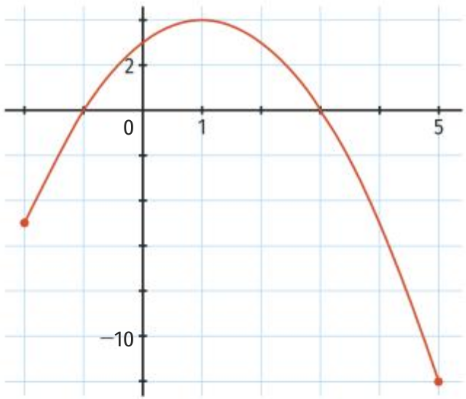
\includegraphics[scale=.25]{exo1.png}
  \end{center}
\end{minipage}
\end{exo}

\begin{exo}~\\[-2mm]
\begin{minipage}{.6\textwidth}
  La courbe ci-contre représente une fonction $g$ définie et dérivable sur
  l'intervalle $I=[-4;2]$.
  \begin{enumerate}
    \item Par lecture graphique, déterminer le sens de variation de $g$ sur $I$.
    \item Donner, suivant les valeurs de $x$, le signe de $g'(x)$ sur
      l'intervalle $I$.
  \end{enumerate}
\end{minipage}
\begin{minipage}{.4\textwidth}
  \begin{center}
    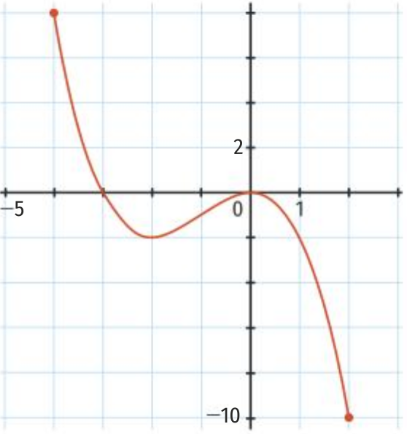
\includegraphics[scale=.25]{exo2.png}
  \end{center}
\end{minipage}
\end{exo}

\begin{exo}~\\[2mm]
\begin{minipage}{.6\textwidth}
  La courbe ci-contre représente une fonction $h$ définie et dérivable sur
  l'intervalle $I=[-2;6]$.
  \begin{enumerate}
    \item Par lecture graphique, déterminer le sens de variation de $h$ sur $I$.
    \item Donner, suivant les valeurs de $x$, le signe de $h'(x)$ sur
      l'intervalle $I$.
  \end{enumerate}
\end{minipage}
\begin{minipage}{.4\textwidth}
  \begin{center}
    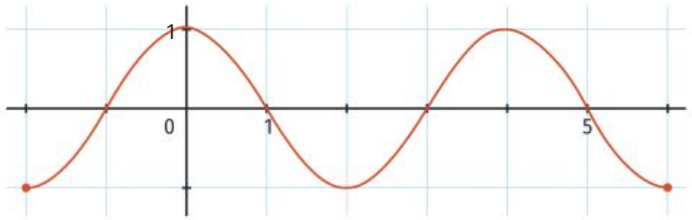
\includegraphics[scale=.25]{exo3.png}
  \end{center}
\end{minipage}
\end{exo}

\begin{exo}
Soit $f$ une fonction définie et dérivable sur
l'intervalle $I=[2;8]$. Le tableau ci-dessous donne le signe de $f'(x)$ sur $I$.
\begin{center}
  \begin{tikzpicture}
  \tkzTabInit{$x$ / .8 , $f'(x)$ / .8}{$2$, $3$, $5$, $8$}
  \tkzTabLine{, +, z, +, z, -}
  \end{tikzpicture}
\end{center}
\begin{enumerate}
  \item Donner le tableau de variations de $f$ sur $I$.
  \item Tracer une courbe susceptible de représenter la fonction $f$.
\end{enumerate}
\end{exo}

\begin{exo}
Soit $g$ une fonction définie et dérivable sur
l'intervalle $I=[0;+\infty[$. Le tableau ci-dessous donne le signe de $g'(x)$ sur $I$.
\begin{center}
  \begin{tikzpicture}
  \tkzTabInit{$x$ / .8 , $f'(x)$ / .8}{$0$, $3$, $6$, $+\infty$}
  \tkzTabLine{, -, z, +, z, -}
  \end{tikzpicture}
\end{center}
\begin{enumerate}
  \item Donner le tableau de variations de $g$ sur $I$, sachant que $g(3)=-1$ et
    $g(6)=2$.
  \item Tracer une courbe susceptible de représenter la fonction $g$.
\end{enumerate}
\end{exo}

\begin{exo}[$\star$]
On pose $f:x\mapsto \sqrt{2x+10}\times(1-x)$.
\begin{enumerate}
  \item Justifier que l'ensemble de définition de $f$ est $I=[-5;+\infty[$, et que
    l'ensemble de dérivabilité de $f$ est $J=]-5;+\infty[$.
    \item Pour $x\in J$, on pose $u(x)=\sqrt{2x+10}$. Calculer, pour $x\in J$,
      l'expression de la dérivée de $u$.
    \item Calculer maintenant, pour tout $x\in J$, l'expression de la dérivée de
      $f$.
    \item Dresser le tableau de signe de $f'$ puis le tableau de variation de
      $f$.
    \item À l'aide de la calculatrice, tracer la courbe représentative de $f$ et
      vérifier vos résultats.
\end{enumerate}
\end{exo}

\begin{exo}
Soit $f$ la fonction définie par
$f(x)=\frac{x^2+3}{x+1}$.
\begin{enumerate}
  \item Préciser l'ensemble de définition et de dérivabilité de $f$, que l'on
    notera $D$.
  \item Calculer, pour $x\in D$, $f'(x)$ puis vérifier que $f'(x) =
    \frac{(x-1)(x+3)}{(x+1)^2}$.
  \item Étudier le signe de $f'(x)$ puis dresser le tableau de variation de $f$
    sur $D$.
\end{enumerate}
\end{exo}

\begin{exo}
\begin{enumerate}
  \item Vérifier que pour tout réel $x$, on a $x^3+3x^2-54 = (x-3)(x^2+6x+18)$.
  \item En déduire le signe du polynôme $P$ défini sur $\mathbb{R}$ par
    $P(x)=x^3+3x^2-54$.
  \item Une entreprise produit $q$ milliers de pièces par jour, $q$ étant un
  réel de $]0;5]$. Le prix de revient d'une pièce, exprimé en euros, dépend de
  $q$ et est donné par l'expression
  \[
    f(q) = \frac{q^3+6q^2+12q+108}{12q}.
  \] 
  \begin{enumerate}
    \item Quel est le prix de revient d'une pièce lorsque l'entreprise produit
      $4200$ pièces par jour ?
  \item Démontrer que pour $q\in]0;5]$, $f'(q)=\frac{P(q)}{6q^2}$ où $P$ est le
    polynôme de la question $2$.
  \item Dresser le tableau de variations de $f$.
  \item En déduire le nombre $q_0$ d'unités à fabriquer pour que le prix de
    revient d'une pièce soit minimal. Quel est alors le montant en euros du coût
    total de production ?
  \end{enumerate}
\end{enumerate}
\end{exo}

\begin{exo}
Au cours d'une montée, le moteur d’un avion s’arrête
brusquement alors que son altitude\\[1mm]
\begin{minipage}[]{.5\textwidth}
est de $2000$ mètres. L’avion suit d’abord une
trajectoire parabolique durant 8 secondes puis le pilote amorce une descente en
vol plané. On se propose d’étudier la première phase de ce vol sans moteur. Dans
la phase où la trajectoire est parabolique, on
\end{minipage}
\begin{minipage}{.5\textwidth}
  \begin{center}
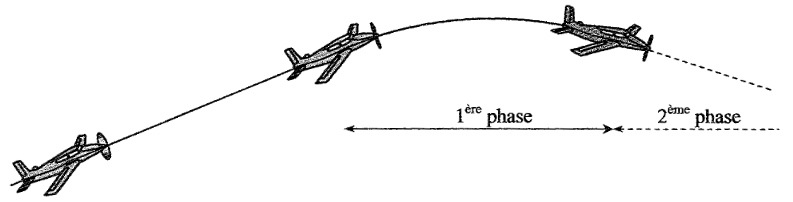
\includegraphics[scale=.3]{avion.png}
  \end{center}
\end{minipage}\\[1mm]
peut définir l'altitude $h$ en mètres de l'avion en fonction du temps $t$ en
secondes par l'expression $h(t) = -0,75t^2+7,5t+2000$ avec $t\in[0;8]$.\\Quelle
est la hauteur maximale de l'avion et son altitude à la fin de la phase
parabolique ? Justifier.
\end{exo}

\begin{exo}
On considère la parabole $\mathscr P$ d'équation
$y=6-x^2$.\\
\begin{minipage}{.75\textwidth}
  \begin{enumerate}
    \item Déterminer les coordonnées des points d'intersection de $\mathscr P$
      avec l'axe des abscisses.
    \item Soit un point $M$ de coordonnées $(x;0)$, où $x\in[0;\sqrt6]$. On
      construit le rectangle $MNPQ$ comme ci-contre où $N$ et $P$ sont sur la
      parabole $\mathscr P$, et où $M$ et $Q$ sont sur l'axe des abscisses.
      Donner les coordonnées de $M$, $N$, $P$ et $Q$.
    \item En déduire la mesure des longueurs $MN$ et $MQ$.
  \end{enumerate}
\end{minipage}
\begin{minipage}{.25\textwidth}
  \begin{center}
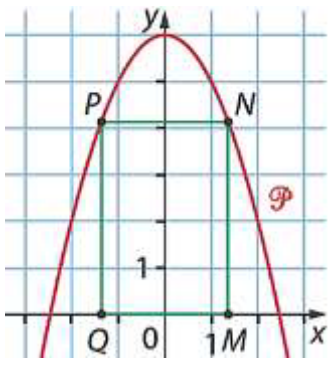
\includegraphics[scale=.3]{parabole.png}
  \end{center}
\end{minipage}
\begin{enumerate}
  \setcounter{enumi}{3}
    \item Déterminer la valeur de $x$ avec une précision à $10^{-2}$ près, pour
      que l'aire de $MNPQ$ soit maximale.
\end{enumerate}
\end{exo}

\begin{exo}
Soit $f$ la fonction définie sur $\mathbb{R}$ par
$f(x)=x^3+3x^2+2x+1$ et soit $\mathscr C_f$ sa courbe\\[1mm]
\begin{minipage}{.75\textwidth}
représentative.
\begin{enumerate}
  \item Calculer $f'(x)$.
  \item Déterminer les variations de $f$, puis dresser son tableau de variations.
  \item Déterminer une équation de la tangente $T$ à la courbe au point
    d'abscisse $-2$.
  \item Le point $S(-4;-3)$ appartient-il à $T$ ?
  \item Vérifier que, pour tout réel $x$, on a $f(x)-(2x+5)=(x+2)^2(x-1)$.
  \item Déterminer la position relative de $\mathscr C_f$ et de $T$ sur
    l'intervalle $[-4;2]$.
\end{enumerate}
\end{minipage}
\begin{minipage}{.25\textwidth}
  \begin{center}
    \begin{tikzpicture}
      \begin{axis}[x=.5cm, y=.5cm, xmin=-3.2, xmax=2.2, ymin=-1.5, ymax=7.5,
        ytick={-1, ..., 7}]
        \addplot[thick, red, samples=101] {x^3+3*x^2+2*x+1};
        \addplot[thick, blue, samples=101] {2*x+5};
      \end{axis}
    \end{tikzpicture}
  \end{center}
\end{minipage}
\end{exo}

\begin{exo}
Soit $f$ une fonction dérivable sur $\mathbb{R}$ et $f'$ sa dérivée. On donne le
tableau de signes de $f'$. La fonction $f$ admet-elle un extremum local ? Si
oui, est-ce un maximum ou un minimum ?
\begin{center}
  \begin{tikzpicture}[scale=.8]
  \tkzTabInit{$x$ / .8 , $f'(x)$ / .8}{$-\infty$, $5$, $+\infty$}
  \tkzTabLine{, +, z, -}
\end{tikzpicture}
\end{center}
\end{exo}

\begin{exo}
Soit $g$ une fonction dérivable sur $]0;+\infty[$ et $g'$ sa dérivée. On donne le
tableau de signes de $g'$. La fonction $g$ admet-elle un extremum local ? Si
oui, est-ce un maximum ou un minimum ?
\begin{center}
  \begin{tikzpicture}[scale=.8]
  \tkzTabInit{$x$ / .8 , $g'(x)$ / .8}{$0$, $3$, $+\infty$}
  \tkzTabLine{, -, z, -}
\end{tikzpicture}
\end{center}
\end{exo}

\begin{exo}
Dans un tronc d’arbre circulaire, on découpe une poutre de forme parallélépipédique rectangle.
La résistance à la flexion de cette poutre varie comme le produit $\ell\times
h^2$ où $\ell =AB$ et $h = BC$ sur la figure ci-
contre. On prend comme unité de longueur, le rayon du tronc d’arbre (ce rayon
vaut donc $1$).\\
\begin{minipage}{.6\textwidth}
  \begin{enumerate}
    \item Montrer que $h^2=4-\ell^2$.
    \item En déduire que $\ell\times h^2=-\ell^3+4\ell$.
    \item On considère la fonction $f:x\mapsto -x^3+4x$ pour $x\geq0$.
      \begin{enumerate}
        \item Étudier le sens de variations de $f$.
        \item Comment choisir $\ell$ et $h$ pour que la résistance de la poutre
          soit maximale ?
        \item Quel est l'angle $\alpha$ correspondant, $0,1$ radian près ?
      \end{enumerate}
  \end{enumerate}
\end{minipage}
\begin{minipage}{.4\textwidth}
  \begin{center}
    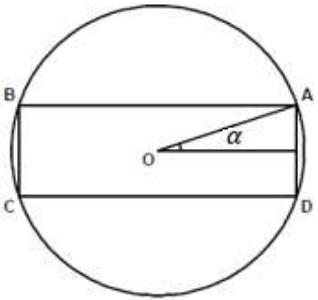
\includegraphics[scale=.4]{poutre.png}
  \end{center}
\end{minipage}
\end{exo}

\begin{exo}
Un industriel doit fabriquer des boîte fermée de volume $1$ L, soit $1$ dm$^3$,
ayant la forme d'un pavé de hauteur $h$ dont la base est un carré de côté $x$.
L'unité de longueur est le dm.
\begin{enumerate}
  \item En vous aidant d'un schéma ou d'un patron de la boîte, justifier que
    $h=\frac{1}{x^2}$.
  \item En déduire que l'aire totale des faces du pavé est
    $S(x)=2x^2+\frac{4}{x}$.
  \item Montrer que pour $x>0$, on a
    \[
      S'(x) = \frac{4(x-1)(x^2+x+1)}{x}
    \]
  \item En déduire les variations de $S$, puis déduire et donner les dimensions
    de la boîte d'aire minimale.
\end{enumerate}
\end{exo}

\begin{exo}
\textbf{Partie A.} Soit $f$ la fonction définie et dérivable sur
$\mathbb{R}\setminus\left\{ -3 \right\}$ par $f(x)=\frac{x^2-ax+b}{x+3}$ où $a$ et
$b$ sont des réels à déterminer. On note $\mathscr C_f$ la représentation
graphique de la fonction $f$, dans un repère orthonormé. On sait que
\begin{itemize}
  \item la courbe $\mathscr C_f$ passe par le point $A\left( 0;
    \frac{4}{3} \right)$.
  \item la tangente de $\mathscr C_f$ au point d'abscisse $1$ est horizontale.
\end{itemize}
\begin{enumerate}
  \item Calculer $f'(x)$ en fonction de $a$ et $x$.
  \item À partir des données de l'énoncé, déterminer les valeurs de $a$ et de
    $b$.
\end{enumerate}
\textbf{Partie B.} On considère maintenant la fonction $f$ définie et dérivable
sur $\mathbb{R}\setminus\left\{ -3 \right\}$ par $f(x)=\frac{x^2-x+4}{x+3}$.
\begin{enumerate}
    \setcounter{enumi}{2}
  \item Calculer $f'(x)$.
  \item Justifier que le signe de $f'(x)$ est donné par le signe du trinôme
    $x^2+6x-7$.
  \item En déduire le signe de $f'(x)$, puis le sens de variation de $f$ sur
    $\mathbb{R}\setminus\left\{ -3 \right\}$.
  \item Déterminer une équation de la tangente $(T)$ à la courbe $\mathscr C_f$
    au point d'abscisse $-2$.
  \item \begin{enumerate}
      \item Calculer l'expression de $f(x)-(-15x+40)$ et montrer que $f(x)\geq
        -15x+40$, pour $x\neq3$.
      \item Étudier les positions relatives de $\mathscr C_f$ et de $(T)$.
    \end{enumerate}
\end{enumerate}
\end{exo}

\end{document}
